\chapter{Circuits}\label{cha:tasks}

XCSoar fournit toutes les fonctionnalités de gestion des circuits sur la campagne. Ils peuvent être édités avant le décollage et modifiés en vol. Le passage au point de virage suivant est automatique. Ce chapitre décrit aussi l'utilisation de l'enregistrement et relecture des vols au format IGC.

Il y a trois modes de circuit:
\begin{description}
\item[Circuit prévu] C'est le mode de circuit normal, dans lequel le circuit est constitué d'un point de départ, de zéro ou plus point de virage et d'un point d'arrivée. Les points doivent être passés dans un ordre défini.
\item[Circuit GoTo] Vol vers un point unique.
\item[Dégagements] Permet de visualiser les terrains posables les plus proches et les informations les concernant, dont l'éloignement et l'altitude nécessaire pour les rejoindre. 
\end{description}

Noter qu'en mode GoTo ou Dégagements le circuit prévu est conservé et peut être repris plus tard. Les données nécessaires aux calculs statistiques relatifs à un circuit accompli sont conservées.

\section{Circuit GoTo}\label{sec:Goto-tasks}

Un circuit Goto peut se définir simplement en sélectionnant un point de virage sur la carte ou bien dans la liste des points de virage ou encore en utilisant: \bmenug{Dégagmts} \blink\bmenug{Aller à} 
\gesture{Bas - Gauche}.  En mode GoTo, la sélection de 
\bmenug{Nav. 2}\blink\bmenug{Circuit Reprendre} permet de revenir au circuit prévu(si il y en avait un).

\subsection*{Goto automatique}

Si aucun circuit n'est prévu (actif) alors au décollage un circuit "Goto" est automatiquement crée avec comme point d'arrivée, le point de décollage ou l'aérodrome le plus proche du point de décollage.

Qu'un circuit soit défini ou pas, le point de décollage est toujours crée automatiquement et apparait dans la liste des points de virage pour pouvoir être utilisé ultérieurement.

\section{Édition des circuits}

Plusieurs méthodes sont possibles. Certaines plus efficaces au sol lors de la préparation du circuit, d'autres utiles pour modifier le circuit en vol lors de vols sur la campagne "touristiques" ou en dehors de compétitions. Les circuits peuvent être crées et sauvegardés sur fichier pour être utilisés plus tard. Ils peuvent être utilisés par toutes les version de XCSoar: sur votre PC vous pouvez donc préparer les circuits de la prochaine saison et les transférer sur l'appareil utilisé dans le planeur, les mettre à disposition pour d'autres vélivoles...

%\tip It is also possible to save a `default' task and have this task loaded
%automatically upon start-up of XCSoar.  One application of this is to
%set up a default task with one waypoint being the home --- this means
%that XCSoar is then programmed for final glide back to home, which is
%useful for casual cross-country touring.

Les principales méthodes de définition des circuits sont:
\begin{itemize}
\item Utilisation de l'interface d'édition de circuit.
\item Sélection de points de virage sur la carte et les ajouter au circuit en utilisant le bouton \bmenug{Détails}.
\item Charger le circuit à partir d'un fichier.
\end{itemize}

%Selecting the Task menu item will produce the Task dialog box.  The
%list box on the left displays all of the turn points loaded into the
%system. Highlight the desired entries and using the "-$>$" and "$<$-"
%buttons assemble the desired task in the Task list box. As each turn
%point is added to the task a continuous display of the calculated task
%length is shown.  Tasks can be saved for recalling later using the
%"Save" button and recalled using the "Load" button.  Once the desired
%task is complete select "OK".
%
%{\it DIAGRAM SHOWING TASK DIALOG EDITING, WITH LABELED ARROWS POINTING
%TO THE USER INTERFACE ELEMENTS?}

\tip Le chargement d'un circuit à partir d'un fichier peut-être très utile pour ceux qui font le même circuit car une seule personne crée le circuit et le distribue ensuite aux autres.

XCSoar sauvegarde le circuit en cours quand le programme est arrêté. A la mise en route le circuit est rechargé. Ceci permet de préparer un circuit tôt dans la journée et d'éteindre l'appareil sur lequel XCSoar fonctionne et de le remettre sous tension juste avant le décollage.

Les points de virage des circuits sont sauvegardés même si le fichier de points de virage est modifié. Ce qui veut dire que si vous sauvegardez un circuit puis changez le fichier de points de virage, et rechargez le fichier de points de virage, de nouveaux points de virage sont crées pour chaque point de virage manquant dans le nouveau fichier.

\section{Informations sur les points de virage}
%Several ways of selecting a waypoint are available:
%\begin{itemize}
%\item Touch its name or the waypoint symbol on the map screen if it is visible.
%\item If the waypoint is in the active task, highlight the waypoint {\InfoBox}, then use the up/down arrow keys to select the desired waypoint, and press the
%enter key.
%\item From the Task dialog, find and highlight the waypoint in
% the waypoint list, then press the 'Details' button.
%\end{itemize}
%The display will now show the waypoint details dialog.

La page des détails des points de virage a des fonctionnalités de navigation comme "Aller à", "Inséré dans le circuit", "Ajouter au circuit" et définir comme nouvelle "base".

On peut y accéder de différentes façons:
\begin{itemize}
\item
Depuis le menu \bmenug{Nav. 1}\blink\bmenug{Circuit}\blink\bmenug{Pts de virage} en sélectionnant un des points de virage du circuit en cours, appuyer dessus une seconde fois pour faire apparaitre la fenêtre de gestion des points de virage, puis utiliser le bouton  \bmenug{Details}.

\item
Depuis \bmenug{Info. 1}\blink\bmenug{Qu'y a-t-il ici?} pour afficher la liste des éléments qui se trouvent sous le curseur ou sous votre doigt sur la carte.

\item
Depuis \bmenug{Nav. 1}\blink\bmenug{Dégagmts} pour afficher les détails des terrains posables les plus proches.

\item
Depuis \bmenug{Nav. 1}\blink\bmenug{Liste des waypoints} pour sélectionner un point de virage dans la liste et afficher ses détails.

\item
Si le point de virage est visible sur la carte, appuyer sur son nom ou son symbole.

\item 
From the menu \bmenug{Nav. 2}\blink\bmenug{Détails Pt de virage} pour afficher les détails du point de virage actif.
\end{itemize}



\subsection*{Détails des points de virage}\label{sec:waypointdetails}
Cette page contient les informations du point de virage: nom aéronautique (LFMR pour BARCELONNETTE Saint-Pons), la fréquence radio, l'axe de piste et sa longueur, coordonnées GPS, altitude, heure du coucher du soleil, cap et distance, différence d'altitude nécessaire pour atteindre ce point avec un calage MC à zéro. Il y a aussi un bouton \button{GoTo} qui permet de démarrer un circuit GoTo vers ce point. L'utilisation de ce bouton, suspend le circuit en cours.

\begin{center}
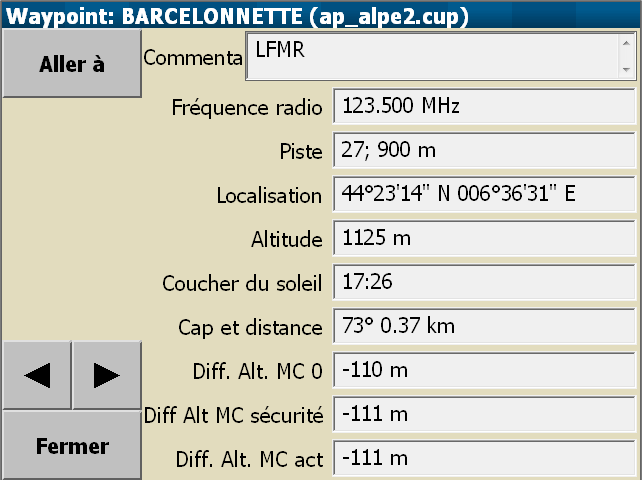
\includegraphics[angle=0,width=0.8\linewidth,keepaspectratio='true']{figures/dialog-waypointdetails0.png}
\end{center}

Cette page contient aussi trois différences d'altitude (altitude en plus, nécessaire pour atteindre, avec sécurité,  le point de virage considéré):
%As mentioned above, the Waypoint info dialog also shows three forms of altitude 
%difference (additional
%altitude required to reach the waypoint at the safety height) for
%the corresponding waypoint:
\begin{description}
\item[Diff. Alt. MC 0] Différence d'altitude nécessaire comparée avec un calage MC à zéro.
\item[Diff Alt MC sécurité] Différence d'altitude nécessaire comparée au calage MC de sécurité. (Voir \ref{sec:secu-parameter} )
\item[Diff. Alt. MC act] Différence d'altitude nécessaire comparée au calage MC actuel.
\end{description}

La page des détails des points de virage est constituées de deux pages (accessibles avec les boutons \button{$>$} et \button{$<$} ). En fonction de l'existence et du nombre d'autres détails propre au point de virage visualisé, d'autres pages pourront être affichées.

\subsection*{Waypoints et Circuit}  
La deuxième page "Détails de points de virage" comporte une colonne de boutons permettant plusieurs actions sur le point de virage étudié:
\begin{description}
\item[\button{Remplacer dans le circuit}] remplace le point de virage actif du circuit en cours par le point de virage sélectionné.
\item[\button{Inséré dans Circuit}] Insère le point de virage sélectionné avant le point de virage actif du circuit en cours.
\item[\button{Ajouter Au Circuit}] Ajoute le point de virage sélectionné à la fin du circuit en cours.
\item[\button{Retirer du circuit}] Retire du circuit en cours le point de virage sélectionné. (option visible seulement si le point de virage sélectionné fait partie du circuit en cours)
\item[\button{Nvelle Base}] Défini le point de virage sélectionné comme nouvelle base de départ.
\item[\button{Panor. au WP}] Passe en mode Panoramique et affiche le point de virage sélectionné.
%\item[\button{Set teamcode}] sets the waypoint as reference waypoint for
%  team code coordinates.


\end{description}

C'est une bonne habitude que de définir votre point "Base" à partir de cette fenêtre de détails des points de virage. XCSoar démarre avec ce point comme  base de départ quand il n'a pas de signal GPS. Quand aucune base n'est définie la base par défaut est le centre de la carte.

\subsection*{Informations Aérodromes}
Cette page peut contenir des extraits des compléments en-route ou autres informations relatives à des points de virage ou des terrains. Pour plus de détails sur le format du fichier contenant ces informations, voir ~\ref{sec:Airfield-details}.

%This page may contain relevant text from the enroute supplement about
%the airfield, including runways, radio frequencies, traffic patterns,
%contacts.
\begin{center}
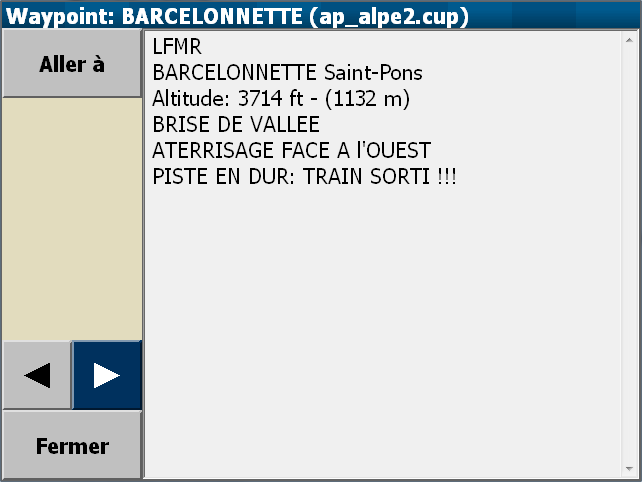
\includegraphics[angle=0,width=0.8\linewidth,keepaspectratio='true']{figures/dialog-waypointdetails1.png}
\end{center}

%\subsection*{Image Satellite}
%Cette page permet d'afficher une vue satellite du point de virage.
%Pour plus de détails sur le format du fichier contenant ces informations, voir ~\ref{sec:Airfield-details}.
%\begin{center}
%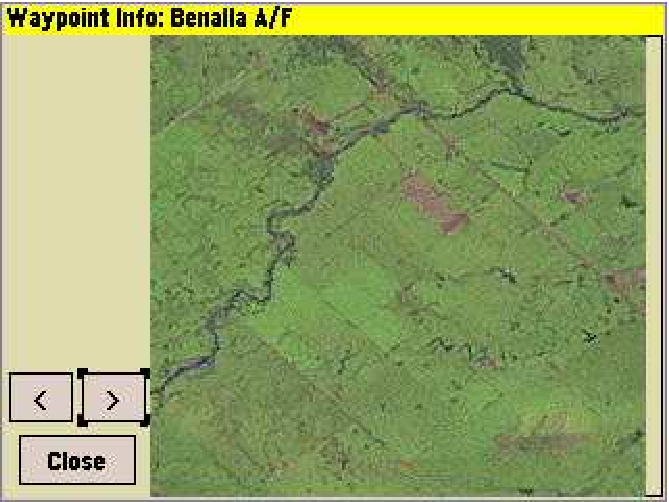
\includegraphics[angle=0,width=0.8\linewidth,keepaspectratio='true']{figures/dialog-waypointdetails2.pdf}
%\end{center}

\section{Sélection des points de virage}\label{sec:waypoint-selector-dialog}
La fenêtre de sélection des points de virage permet de retrouver un point de virage dans une liste pouvant être très importante. 

On y accède de plusieurs façons:
\begin{itemize}
\item depuis  \bmenug{Nav. 1}\blink\bmenug{Liste des waypoints}
\item depuis l'éditeur de circuits,  \bmenug{Nav. 1}\blink\bmenug{Circuit} et "Général" et créer un nouveau circuit et ajouter un point de virage.
\item ou simplement par geste(le plus rapide)\gesture{Bas - Droit}.
\end{itemize}

Le sélecteur de points de virage comporte sur la gauche plusieurs filtres optionnels qui peuvent être combinés. Les résultats sont à droite. 
\begin{description}
\item[Nom] Tri basé sur les premières lettres du nom du point recherché. Au fur et à mesure que les caractères du nom sont choisis, la liste affichée se réduit pour faciliter la sélection.\\
\item[Distance] Affichage des waypoints se trouvant à l'intérieur d'un cercle, centré sur le planeur, dont on défini le rayon.\\
\item[Direction] Affichage des waypoints qui sont dans un cap défini par rapport au planeur.
 Une direction spéciale "HDG(125°)" montre les waypoints qui sont dans les 30° de part et d'autre de la route du planeur (ici route au 125). Ceci permet au pilote de répertorier rapidement les terrains se trouvant dans la direction qu'il suit.\\
\item[Type] Affiche les waypoints qui sont du type choisi (posable, aérodrome, point de virage) ou qui sont dans le fichier principal de waypoints ou dans le fichier secondaire ou parmi ceux récemment utilisés.\\
\end{description}
Quand on tri par nom et par type le résultat est classé par ordre alphabétique. Quand (en plus) on tri par distance ou direction le résultat est classé par distance.

\begin{center}
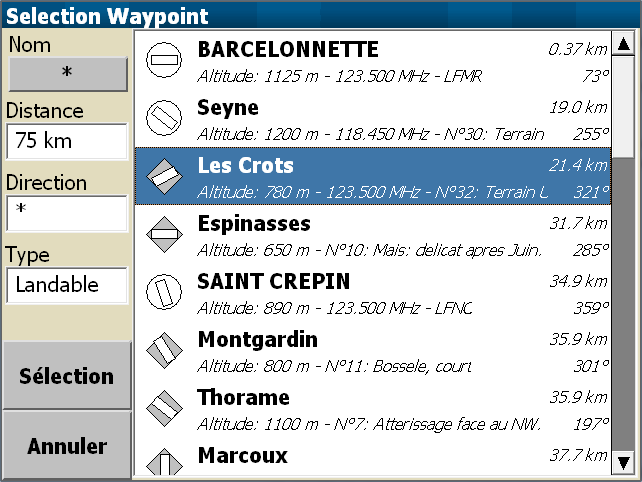
\includegraphics[angle=0,width=0.8\linewidth,keepaspectratio='true']{figures/dialog-waypointselect.png}
\end{center}

Si la liste de résultats est longue, on peut la faire descendre ou monter à l'aide de l'ascenseur de droite. 

La sélection d'un des éléments de la liste conduit à un comportement différent suivant la fonctionnalité qui à été utilisée précédemment. Le cas le plus courant est l'ouverture de la fenêtre de détails du point choisi. 

\section{Gestionnaire de circuit}\label{sec:task-manager-dialog}
\begin{it}  La gestion des circuits à subit une refonte importante. De notables différences et nouveautés sont donc apparues en comparaison aux précédentes versions de XCSoar.\end{it}

Le gestionnaire des circuits permet d'éditer, voir, charger, modifier, sauvegarder sur fichier et déclarer les circuits. On y accède par le menu
\begin{quote}
\bmenug{Nav. 1}\blink\bmenug{Circuit}
\end{quote} 

La première page du gestionnaire de circuit montre divers calculs relatifs au circuit en cours, comme expliqué en détails après. Il y a en plus les onglets   \button{Calculateur}, \button{Pts de virage}, \button{General}, et  \button{Règles}, et aussi un onglet pour \button{Fermer} le gestionnaire de circuit.

\subsection*{Points de virage}
L'onglet \button{Pts de virage} affiche une liste ordonnée des points de virages du circuit en cours. Si il n'y a pas de point de virage dans le circuit,  "(Ajouter point de virage)" est affiché. En sélectionnant cette ligne le sélecteur de points de virage apparait comme décrit précédemment. Le choix d'un point de virage l'ajoute au circuit en cours de création.

\subsection*{General}
En appuyant sur \button{General} quatres boutons peuvent être sélectionnés:

\begin{itemize}
\item \button{Nouveau circuit} Efface le circuit courant de la mémoire de travail. Les valeurs des règles sont les valeurs par défaut.
\item \button{Déclarer}  Si un logger externe est connecté, ceci permet de charger le circuit actif vers le logger et de le déclarer.
\item \button{Circuits enregistrés} Affiche la liste des circuits enregistrés. Un circuit déjà préparé et sauvegardé, peut être utilisé. Il faut noter que le circuit actif courant est remplacé par le circuit choisi.
\item \button{Enregistrer}  Sauvegarde du circuit actif courant. En appuyant sur \button{Enregistrer} un nom de fichier devra être donné: un nom explicite est de bonne augure pour pouvoir le retrouver ensuite dans la liste des circuits existants.
\end{itemize}

\subsection*{Règles}
Les champs affichés en appuyant sur  \button{Règles} dépendent du type de circuit choisi. En sélectionnant un champ, une fenêtre apparait pour permettre de modifier la valeur de ce champ. Les types de circuit sont expliqués en détails juste après.

En appuyant sur \button{Règles} quand il est en bleu, une vue générale de la carte apparait avec le tracé du circuit.

\subsection*{Type de circuit}
XCSoar pour le moment supporte trois types de circuits: Course, AAT et Insignes/records FAI

Une description sommaire de ces types de circuit est faite dans ce manuel. Cependant la définition exacte et à jour de ces types de circuit, si elle vous intéresse, doit être recherchée  dans les documents officiels. Les règlements FAI sont sur  \url{http://www.fai.org/fai-documents}. 

\begin{itemize}
\item Course (course sur circuit).  passage obligatoire à chaque point de virage défini, et dans l'ordre fixé. Le choix de ce type d'épreuve permet de définir les valeurs des champs suivants (note: si l'option "Règles de départ/arrivée FAI" est mise à On alors aucunes de ces options sont disponibles):
  \begin{itemize}
  \item Vitesse max. au départ: C'est la vitesse maxi au passage de la ligne de départ. Si la vitesse n'est pas limitée, il faut mettre 0.
  \item Hauteur max. départ : hauteur maxi au passage de la ligne de départ. C'est la hauteur maxi au-dessus de la hauteur de départ de référence(AGL ou MSL) autorisée pour l'épreuve. Si pas de limite, il faut mettre 0.
  \item Hauteur départ réf. : défini si la hauteur maxi du point de départ est au dessus du sol (AGL) ou bien au-dessus du niveau moyen de la mer (MSL). AGL = QFE et MSL = QNH.
  \item Hauteur min. arrivée: hauteur minimum de passage au-dessus de la ligne d'arrivée. Hauteur basée sur le type de référence de hauteur d'arrivée (AGL ou MSL). Si pas de limite, il faut mettre 0.
  \item Ref. hauteur arrivée: défini si la hauteur mini du point d'arrivée est au dessus du sol (AGL) ou bien au-dessus du niveau moyen de la mer (MSL).
  \item Règles de départ/arrivée FAI: sur On, le pilote doit connaitre les règles FAI adaptées au type de circuit et de record qu'il souhaite réaliser. 
  \end{itemize}
\item AAT (épreuve de vitesse sur secteurs). Circuit limité en durée. Passage par des zones cylindriques ou non et dans l'ordre défini. Les champs de valeurs à remplir sont:
  \begin{itemize}
  \item Temps mini AAT: temps minimum requis (en minutes) pour l'épreuve. Se référer aux documents officiels pour plus de détails, surtout pour le calcul des pénalités lors de l'arrivée avant le temps minimum imparti.
  \item Vitesse max. au départ: idem que pour "Course sur circuit".
  \item Hauteur max. départ : idem que pour "Course sur circuit".
  \item Hauteur départ réf. : idem que pour "Course sur circuit".
  \item Hauteur min. arrivée : idem que pour "Course sur circuit".
  \item Ref. hauteur arrivée : idem que pour "Course sur circuit".
   \item Règles de départ/arrivée FAI : idem que pour "Course sur circuit".
 \end{itemize}
\item Insignes/records FAI :  ce type de circuit ne permet que des départs, arrivées et points de virage de type FAI. Ceci pour l'obtention d'insigne/record FAI. Permet l'utilisation de l'altitude d'arrivée FAI lors du calcul du plan d'arrivée.
\end{itemize}

Une fois sélectionnés, les points de virage peuvent être déplacés avec les flèches Haut et Bas. Le point de virage de début est automatiquement un point de type "Départ" et celui du bas le point de type "arrivée".

Quand le type de circuit a été choisi et que les règles de départ et d'arrivée ont été définies, il faut préciser les propriétés des points de virage. Les points de virage peuvent être aussi des points de départ ou d'arrivée.\\
Ceci se fait en appuyant sur  \button{Pts de virage} du gestionnaire de circuit. Choisir un des points de virage de la liste (si il y en a de définis). Appuyer 2 fois sur le point de virage désiré ou un fois puis sur \button{Editer le point} le panel d'édition des points de virage apparait. En appuyant sur  \button{Modifier le type} on obtient la liste des différents types de points de virage possibles. Un rappel de la définition du point et de sa spécificité se trouve en bas de la liste. 
L'interface utilisateur permet de comprendre rapidement la signification des différents boutons disponibles ainsi que des champs pouvant être modifiés. Un schémas représentant le type de point choisi facilite aussi la compréhension. 

\section{Démarrage du circuit}\label{sec:demarrage-circuit}

Une fois que les waypoints sont bien définis (départ, points de virage et leur particularités, arrivée) ainsi que les règles du circuit, il reste deux choses à faire:
\begin{itemize}
\item  \button{Enregistrer} pour sauvegarder le circuit en lui donnant un nom, ou si vous venez de modifier un circuit existant, lui donner le même nom ou un autre nom si vous souhaitez en créer un nouveau à partir d'un existant.
\item Appuyer sur l'onglet  \button{Fermer} du gestionnaire de circuit. Suivant les créations, modifications faites auparavant, les dialogues qui apparaissent sont différents. Vous pouvez annuler les modifications afin de garder le circuit en cours. Vous pouvez choisir  \button{Vol} pour utiliser le circuit que vous venez de modifier ou de créer. Le bouton  \button{Annuler les modifications} permet d'oublier les modifications faites et de continuer avec le circuit qui était chargé précédemment. Si vous avez crée un nouveau circuit et que vous l'avez enregistré, il n'est pas perdu, vous le retrouverez plus tard dans la liste des circuits: par contre le circuit qui était en cours, lui, a bien été effacé de la mémoire de travail. Il vous faut donc recharger le circuit que vous souhaitez réaliser.
 \end{itemize}

Si vous avez appuyé sur  \button{Vol} le circuit est démarré (actif).

\section{Déroulement et faux départs}\label{sec:advanc-rest-tasks}
A chaque instant un point de virage est désigné comme point de virage "actif" : c'est celui vers lequel on se dirige, le prochain dans la liste des waypoints du circuit. Le waypoint actif est utilisé pour les calculs et l'affichage des informations de navigation. Le pilote est dirigé vers le point "actif" : voir le chapitre ~\ref{cha:infobox}.

En vol, l'affichage de la direction à suivre pour atteindre le point actif, est permanent.

L'altitude requise pour terminer le circuit est calculée à partir de la position du planeur par rapport au waypoint actif jusqu'au point d'arrivée.

Le passage au point de virage suivant est automatique ou manuel. 
Pour les points de départ en compétition, le passage de ligne se fait plus d'une fois, avant ouverture de ligne ou pour ruser (ou essayer de ruser) et faire un faux départ.

\tip Conseil pour les  utilisateurs de XCSoar en compétition: lors du véritable passage de ligne, il faut vérifier que  \bmenug{Nav. 1}\blink\bmenug{Point de virage précédent} n'est pas sélectionnable et que après avoir passé la ligne, le message de passage de ligne est bien apparu avec \bmenug{Info. 3}\blink\bmenug{Répéter message} ou bien en vérifiant votre objectif avec \bmenug{Nav. 1}\blink\bmenug{Circuit}\blink\bmenug{Objectif} ou plus simplement en vérifiant que la flèche vous donnant le cap à suivre ne pointe pas vers la ligne de départ!!
 Pour repasser la ligne après un ou plusieurs passages (faux départ, passages multiples avant l'ouverture de ligne) le bouton \bmenug{Nav. 1}\blink\bmenug{Point de virage de départ} doit être utilisé pour que le calculateur vous donne la route à suivre vers la ligne de départ.\\
Les points de virages des AAT sont des cas spéciaux qui demandent d'être "armé" avant que calculateur passe au point de virage suivant car c'est le pilote qui décide si il a bien été passé. Pour tous les autres types de waypoint le passage au point suivant est automatique, une fois qu'il a bien été passé.

Pour des circuits "touristiques" il n'y a donc pas d'interaction nécessaire lors du passage des points de virage. Quand un point de virage est atteint, le système passe automatiquement au suivant. Manuellement, le pilote peut toujours avancer ou reculer le point de virage "actif" avec \bmenug{Nav. 1}\blink\bmenug{Point de virage précédent} et \bmenug{Nav. 1}\blink\bmenug{Point de virage suivant} respectivement.

Le contenu des boutons \bmenug{Point de virage précédent}  et \bmenug{Point de virage suivant} est dynamique: ils indiquent l'action qui sera faite si on appuie dessus.

Pour les points de virage nécessitant une "préparation" ou un "armement", \bmenug{Nav. 1}\blink\bmenug{Point de virage suivant}  devient \bmenug{Préparer virage} si le point de virage n'est pas "préparé"; si il est préparé, alors il se change en \bmenug{Point de virage suivant} permettant l'avance manuelle.   \bmenug{Nav. 1}\blink\bmenug{Point de virage précédent} devient  \bmenug{Désarmer le virage} si le waypoint est préparé; si il n'est pas préparé, alors il devient \bmenug{Point de virage précédent} permettant le passage manuel au point précédent.

Des messages apparaissent pour les points nécessitant une préparation, une fois dans la zone définie pour le point actif. Ce sont des rappels au pilote de préparer le passage du waypoint quand il est prêt à passer au point de virage suivant. 

Pour les PC et Pocket PC avec écran tactile uniquement, l'utilisateur peut passer manuellement d'un point à l'autre en sélectionnant le waypoint {\InfoBox}  et en appuyant sur les touches Haut et Bas.

Voir ~\ref{sec:task-rules} pour plus de détails concernant le passage des zones ou points de virages. 

Si le pilote passe les points de virage manuellement, cela ne signifie pas qu'il les a passé réellement! Mais cette fonctionnalité est utile pour forcer un nouveau départ ou bien pour sauter un point de virage quand on ne fait pas de compétition.

\tip Le départ des circuit peut être redémarré simplement en revenant manuellement au point de départ.

Dans tous les types de circuit, si le planeur entre plusieurs fois dans la zone de départ ou bien passe plusieurs fois la ligne de départ, le circuit est redémarré automatiquement.

En sélectionnant \button{Point de virage précédent} le système "oubli" que ce point de virage a déjà été passé: le gestionnaire de circuit s'attend alors à devoir repasser par ce point de virage pour pouvoir terminer le circuit comme défini au départ. Le pilote peut toujours appuyer sur \button{Point de virage suivant} pour définir le prochain point de virage.

Un message associé d'une alarme sonore apparait à chaque passage au point suivant. Les messages sont affichés quand le système avance automatiquement au prochain point  ou en mode "préparé manuel, quand le waypoint est préparé et le planeur dans le secteur du point de virage:
\begin{itemize}
\item[Démarrage circuit]  apparait au passage de la ligne ou à la sortie du secteur de départ: le nombre de passages n'est pas limité.
\item[Dans le secteur,]  armer point suivant quand vous voulez! Ce message apparait à l'entrée de la zone de point de virage. La préparation se fait juste avant de passer le point de virage: c'est simplement pour déclarer au système que le point est passé et que l'on se dirige vers le point de virage suivant. Si le pilote souhaite allonger sont passage dans la zone et qu'il a déjà "préparé" le waypoint, il lui suffit de revenir en arrière en appuyant sur \button{Désarmer} si il a préparé le point suivant ou bien \button{Point de virage précédent}.
\item[Circuit terminé]  Ce message apparait lors du passage de la ligne ou du cylindre d'arrivée. 
\end{itemize}

\section{Règles du circuit}\label{sec:task-rules}

Un certain nombre de règles peuvent être utilisées lors de la définition du circuit, dont les triangles FAI et les AAT. Un grand nombre des paramètres de ces règles peuvent être ajustés.

Les lignes de départ et d'arrivée sont centrées sur leur point de virage associé. Les lignes sont respectivement perpendiculaires aux routes de départ et d'arrivée.

Les secteurs de points de virage des épreuves FAI sont prédéfinis, ainsi que ceux de la BGA britannique et les secteurs DAeC Allemands.

Les conditions de validité du départ dépendent du type de départ :
\begin{description}
\item[Cylindre de départ] Quand le planeur quitte la surface du cercle.
\item[Ligne de départ] Quand le planeur passe la ligne en direction du premier point de virage.
\end{description}

Les conditions de validité de passage des points de virage intermédiaires dépendent de leur type :
\begin{description}
\item[Quadrant FAI] Passage valable quand le planeur passe au-dessus d'une zone définie par un quart de cercle de 20 km de rayon, centré sur le point de virage et centré sur la bissectrice de l'angle.
\item[Secteur DAeC] Règles Allemandes. Passage valable si dans un cercle de 0.5 Km autour du point de virage et dans un secteur de 90° centré sur la bissectrice de l'angle et de 10 Km de rayon.
\item[Cylindre de point de virage]  Passage valable si survol de la surface au sol du cylindre centré sur le point de virage.
\item[Épreuve de type BGA]  Règles britanniques. Passage valable si dans un cercle de 0.5 Km autour du point de virage et dans un secteur de 90° centré sur la bissectrice de l'angle et de 20 Km de rayon.
\item[Épreuve de type BGA avec options] Règles britanniques. Passage valable si dans un cercle de 0.5 Km autour du point de virage et dans un secteur de 180° centré sur la bissectrice de l'angle et de 10 Km de rayon.
\item[Zone secteur de cercle (AAT)]  Passage valable si dans un cercle, ou portion de cercle, centré sur le point de virage. 
\item[Zone secteur de couronne (AAT)]  Passage valable si dans une couronne, ou portion de couronne, centré sur le point de virage. 
\end{description}

La validité du passage du point d'arrivée dépend de son type :
\begin{description}
\item[Cylindre d'arrivée] Passage valable quand le planeur entre dans une zone cylindrique centrée sur le point d'arrivée.
\item[Ligne d'arrivée] Quand le planeur passe un segment centré sur le point d'arrivée et perpendiculaire à la route reliant le dernier point de virage et le point d'arrivée.
\end{description}


Les règles de compétition peuvent être définies dans un fichier de profil et distribué à une équipe ou à l'ensemble des\tip concurrents pour qu'ils puissent concourir avec les mêmes règles!

Des règles spécifiques aux points de départ et d'arrivée peuvent aussi être définies. Une hauteur maxi au-dessus du sol et une vitesse maxi pour les départs. Une hauteur minimum au-dessus du sol pour les arrivées. Ces paramètres sont modifiables dans le menu\config{taskrules}  \bmenug{Config. 2}\blink\bmenug{Options Système} dans l'onglet "Valeurs par défaut du circuit".

Pour les circuits qui ne sont pas des AAT, une option es t disponible afin de paramétrer l'altitude minimum d'arrivée, en accord avec les règles FAI. Dans ce cas, l'altitude d'arrivée peut être inférieure à celle de départ de moins de 1000 mètres au maximum.

\section{Points de départ mulitiples}\label{sec:alternate-starts}

Les points de départ multiples ne sont plus supportés par XCSoar 6.0 mais pourraient être de retour dans de prochaines versions.
%Alternate start points are skipped for XCsoar 6.0, but
%will potentially brought back in a next release. 

%\todonum[inline]{Alternate start points are skipped for XCsoar 6.0, but
%will potentially brought back in a next release. This section can thus be
%treated as obsolete. }

%The task system allows alternate start sectors to be defined.
  
%To use it, on the task edit page, select the start point, then turn on
%the `Alternate start points' property.  Then press the button 'Edit
%alternate start points'.

%\begin{center}
%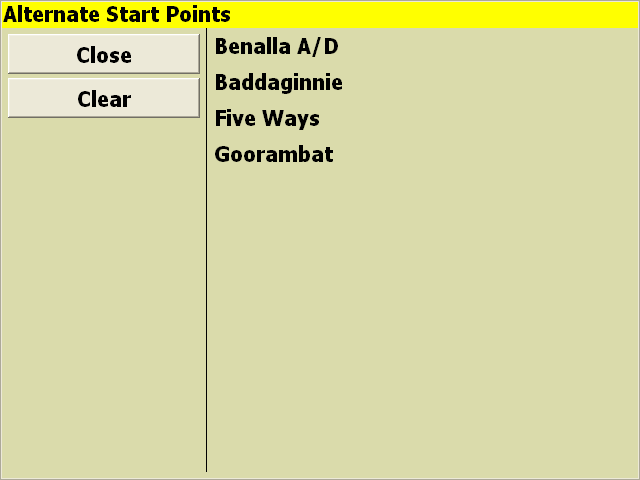
\includegraphics[angle=0,width=0.8\linewidth,keepaspectratio='true']{figures/dialog-startpoint2.png}
%\end{center}
  
%  To edit the start points, move the cursor to an item in the list on
%  the right side of the dialog, and press enter.  This opens the
%  waypoint selector dialog, to allow selection of the waypoint.  This
%  process can be repeated several times for several alternate start
%  waypoints.  Press the `clear' button to clear all alternate start
%  points.

%  Each start sector is fixed to the same type (line/cylinder) and size
%  (start radius) defined in the task waypoint page.

%  Note that the task start point should be included in the alternate
%  start location list. 

%\begin{center}
%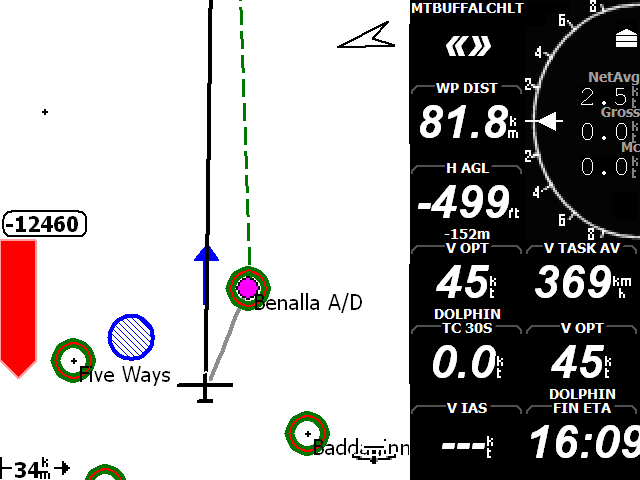
\includegraphics[angle=0,width=0.8\linewidth,keepaspectratio='true']{figures/dialog-startpoint3.png}
%\end{center}

%\begin{center}
%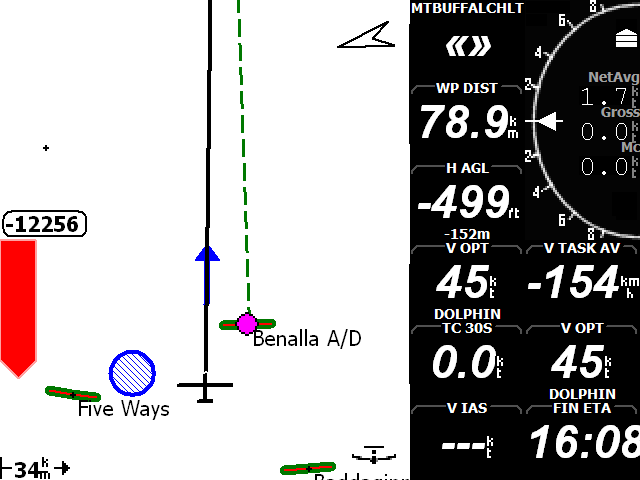
\includegraphics[angle=0,width=0.8\linewidth,keepaspectratio='true']{figures/dialog-startpoint4.png}
%\end{center}

%  In flight, any time you cross a start line (or exit a start
%  cylinder), this will start the task at that particular alternate
%  start.  Task statistics are recalculated for the start sector you
%  last flew through.  All alternate start sectors are shown on the
%  map.  You can re-start simply by flying through the start sector
%  again or another start sector.  This automatic re-start will only
%  happen if the active waypoint is the first turnpoint after the
%  start, or the start itself.

%  When the waypoint advance mode is `Arm' or `Arm Start', then a start
%  is only recognised by XCSoar if the advance trigger is armed.

%  If desired, alternate start points may be selected as the active
%  waypoint by selecting the previous waypoint.  Continuing to select
%  the previous waypoint will cycle through all alternate start points.

\section{Circuit et ergonomie}\label{sec:task-calc-dial}
L'ergonomie de l'interface permet au pilote de visualiser rapidement les effets, sur la performance finale, des modifications qu'il lui sont possible d'affecter à deux paramètres.

C'est accessible de plusieurs façons : \gesture{Droite - Bas}
\begin{itemize}
\item Par geste sur la carte
\item A partir du menu 
\begin{quote}
\bmenug{Nav. 1}\blink\bmenug{Circuit}
\end{quote}
\item Depuis le menu \bmenug{Info 1}\blink\bmenug{Analyses} et en appuyant sur \button{Calc. circuit}
\end{itemize}

\begin{center}
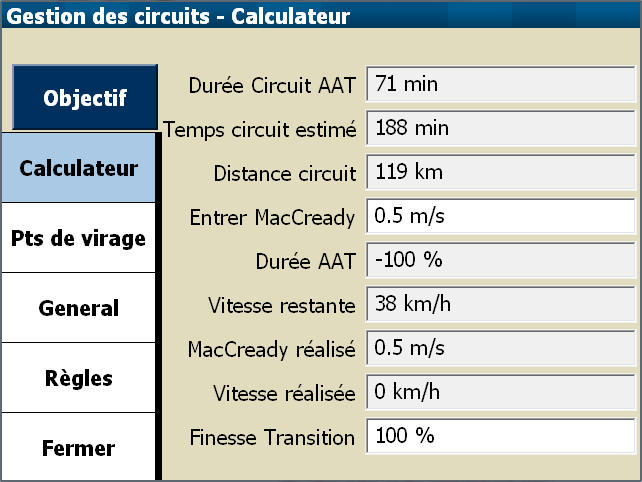
\includegraphics[angle=0,width=0.8\linewidth,keepaspectratio='true']{figures/dialog-taskcalc3.png}
\end{center}

\begin{description}
\item[Durée Circuit AAT]  Durée imposée du circuit.
\item[Temps circuit estimé]  Temps total estimé pour terminer le circuit en tenant compte du calage MC.
\item[Distance circuit]  Distance restante pour terminer le circuit.
\item[Entrer MacCready]  Permet au pilote de faire varier le calage MacCready et d'observer son influence sur le temps estimé du circuit.
\item[Durée AAT]  Pour les épreuves AAT. Représente la performance de votre vol basée sur les données de l'épreuve, par rapport au plus grand et plus petits circuits possibles. -100 \% représente le plus petit circuit possible, 0 \% le circuit nominal et +100 \% le plus grand circuit.
\item[Vitesse restante]  Cette vitesse est la vitesse estimée pour le reste du circuit tenant compte du calage MC donné.
\item[MacCready réalisé]  This field displays the achieved MacCready value.
\item[Vitesse réalisée]  Calage MacCready réalisé.
\item[Finesse Transition]  100 \% indique une performance égale au calage MC. Plus de 100 \% pour un performance supérieure à celle du calage MC (ex : sous des rues de nuage) et mois de 100 \% si vous êtes souvent à côtés de vos pompes... Ce paramètre évalue la performance du vol en croisière en fonction de l'historique du vol avec le calage MC. Les calculs démarrent à partir du passage de la ligne de départ.
\end{description}
Regarder la section~\ref{sec:task-speed-estim} pour plus de détails concernant les calculs des vitesses.

En fermant la fenêtre la valeur du calage MacCready est utilisée comme calage MC pour les calculs. 
%On closing the dialog the entered MacCready value is used as the MacCready 
%setting. If the \button{Cancel} button is pressed, the MacCready setting is 
%unaffected.

Pour les AAT le bouton \button{Objectif} ajuste la distance (en plus ou en moins) de sorte que le temps estimé soit supérieur au temps imparti de 5 minutes maximum. La distance est ajustée en fonction des points objectifs restants. En utilisation standard, tous les objectifs sont réglés sur "Optimisé" ce qui fait que le pilote n'a pas à s'occuper de positionner manuellement les points objectif pour trouver la meilleure distance à parcourir dans le temps imparti. Il peut donc se consacrer à autre chose pendant ce temps.
%The \button{Target} button, for AAT tasks, adjusts the range
%(increases or decreases) so that the estimated task time exceeds the
%assigned task time by less than five minutes.  The range is adjusted
%target-wise. In typical use, all targets are set to ``auto" that means the pilot 
%does not have to manually adjust the range to find the course for arrival at 
%the assigned task time, thereby reducing pilot workload.


\section{États du circuit}\label{sec:task-status}

Cet ensemble de pages permet d'accéder rapidement aux principales informations concernant le circuit en cours. Elles sont utiles pour avoir une vue générale des données du vol et permettent de libérer des InfoBox pour afficher d'autres paramètres. On y trouve la confirmation de la validité du passage de la ligne de départ et des informations de progression du circuit. On y accède part le menu:
\begin{quote}
\bmenug{Info. 2}\blink\bmenug{Etats}
\end{quote}

L'onglet 'Task' récapitule: la rurée AAT impartie, le temps estimé du circuit, le temps restant, la distance parcourue et la distance restante la vitesse estimée et la vitesse moyenne.\\
L'onglet 'Rules' donne la validité des points de départ et d'arrivée en accord avec les règles du circuit.
\begin{center}
\begin{tabular}{c c}
Task & Rules \\
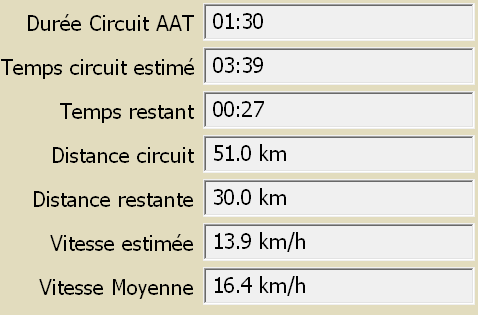
\includegraphics[angle=0,width=0.4\linewidth,keepaspectratio='true']{figures/status-task.png} &
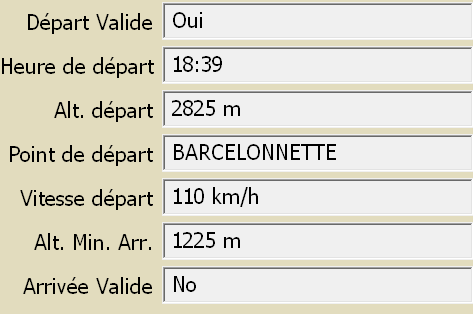
\includegraphics[angle=0,width=0.4\linewidth,keepaspectratio='true']{figures/status-rules.png} \\
\end{tabular}
\end{center}

\section{Assigned Area Tasks : AAT}\label{sec:aat-tasks}

\subsection*{Objectifs AAT}

Un {\em Objectif} pour les AAT, est un point dans une zone de virage AAT vers lequel le pilote se dirige pour optimiser son épreuve. Ces objectifs peuvent être déplacés à l'intérieur des zones afin d'ajuster au mieux la distance du circuit par rapport au temps imparti. Les objectifs peuvent être positionnés avant le vol, pendant la préparation du circuit et modifiés en cours d'épreuve.

Au cours d'un AAT, le calculateur dirige le planeur vers l'objectif. Les statistiques comme la distance au waypoint sont calcules à partir de l'objectif, non pas à partir du point de virage de la zone de l'AAT lui même.

L'avance automatique au prochain point de virage n'est pas déclenchée seulement en entrant dans la zone AAT. Le pilote doit "préparer" le passage au point de virage suivant lui même, manuellement. En faisant cela l'optimiseur de circuit est mis en route afin de relever les coordonnées du point de virage réalisé et mettre à jour les données pour le calcul de l'optimisation du reste du circuit. Voir section ~\ref{sec:advanc-rest-tasks} pour plus de détails.

\subsection*{Déplacement manuel des objectifs}
Dans le but de simplifier le positionnement des points objectifs, le paramètre "Durée AAT" permet de connaitre l'amplitude de la longueur du circuit défini par rapport aux distances minimum et maximum possibles. Si ce paramètre affiche 100\% la position des objectifs donne le plus grand circuit possible. Si il affiche ~$-100$\% c'est alors le plus petit circuit possible. 

Une valeur de zéro représente le circuit nominal : pour des zones en forme de secteur, l'objectif se trouve au milieu de la bissectrice, pour des zones cylindriques, il est au centre.

Les objectifs peuvent être déplacés un par un à l'aide du panel \bmenug{Objectif} et des flèches permettant de passer de l'un à l'autre.\\

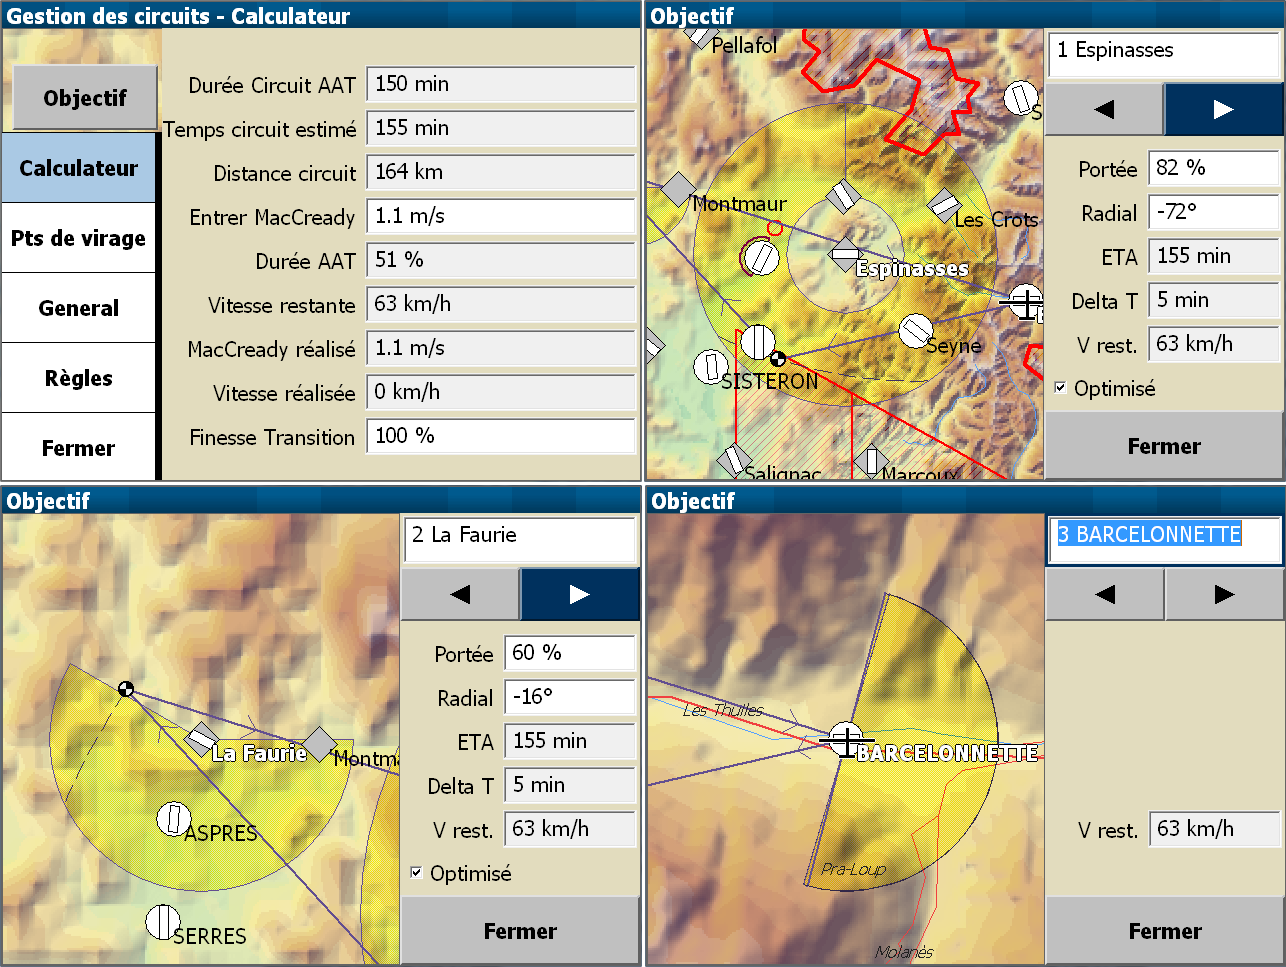
\includegraphics[angle=0,width=1.2\linewidth,keepaspectratio='true']{figures/gestion_circuit_00.png}

Dans la fenêtre "Objectif" si la case "Optimisé" est cochée, la position de l'objectif est calculée par l'optimiseur.

\subsection*{Objectifs AAT et calculateur}

Déroulement classique d'une épreuve AAT avec utilisation des objectifs :
\begin{itemize}
\item entrer les valeurs des paramètres MC, moucherons, ballast, force et direction du vent en utilisant "Options Vol" et "Options Vent".
\item Définir le circuit avec l'éditeur de circuits.
\item En se basant sur son jugement et sur son expérience, en fonction de la météo du jour, de sa connaissance de la région, le pilote peut placer un par un les objectifs de chaque zone de virage (\bmenug{Nav. 1}\blink\bmenug{Circuit}\blink\bmenug{Objectif}). Le paramètre ETA permet d'avoir une idée de la durée estimée du vol et de la comparer à la durée impartie de l'épreuve. Le paramètre Delta T permet de contrôler si la variation de position de l'objectif est efficace ou non.
\item En vol, si les conditions changent et que le calage MC est modifié ou que le vent estimé est modifié, le gestionnaire de circuit peut être ouvert pour vérifier la valeur de la durée estimée du vol.
\item Si le pilote décide d'allonger ou de réduire le circuit, les objectifs des points de virages restant peuvent être repositionnés à l'aide de l'éditeur de circuit.
\end{itemize}

Le calculateur aide ainsi le pilote à répondre à la question "que se passera-t-il si ?", par exemple :
\begin{itemize}
\item Que se passera-t-il si les conditions s'améliorent? Le calage MC peut-être augmenté et le pilote peut voir si il y a assez de distance restante pour agrandir son circuit dans les limites imposées. 
\item Que se passera-t-il si les contritions se dégradent? Le calage MC peut-être réduit et le pilote peut voir si il y a assez d'espace dans les zones pour diminuer son circuit dans les limites imposées tout en passant la ligne d'arrivée juste après la durée imposée.
\item Que se passe-t-il si je quitte la zone AAT maintenant? En appuyant sur \button{Préparer virage} la prise en compte de la position courante par l'optimiseur de circuit est forcée et les paramètres calculés sont mis à jour comme si on avait viré. La position des objectifs suivant peut-être visualisée avec \bmenug{Objectif}.
\end{itemize}

\subsection*{Position de l'objectif}

XCSoar analyse en permanence le chemin du planeur dans les zones AAT pour calculer les waypoints théoriques donnant le score maximum pour la distance parcourue effective. En interne, le programme bouge les points de virage des zones passées qui sont alors les points de virage optimum. 
%XCSoar continually analyses the path of the glider through AAT sectors
%to find the points in previous AAT sectors through which the achieved
%scoreable distance will be greatest.  Internally, the program moves
%the targets for previous AAT sectors, which are then the optimal
%targets.

Dans certains cas l'objectif de la zone AAT active peut-être déplacé automatiquement :
\begin{itemize}
\item Quand à l'intérieur de la zone, l'objectif est projeté sur la droite passant par l'objectif de la zone précédente et la position actuelle du planeur. Ceci permet au pilote de continuer sur la même route et d'avoir un objectif optimisé sur sa route.  
%When inside an AAT sector, the target in that sector is moved to
%to a line projecting from the previous sector's target through the
%aircraft, at the same distance from the previous sector's target to
%the target prior to entering the sector.  The effect of this is to
%allow pilots to choose to enter an AAT sector in a different direction
%or offset from the direct line from the previous target to the current
%target.
\item Quand le planeur est dans la zone AAT, que la distance au dernier objectif est supérieure à la distance au prochain objectif, alors l'objectif est projeté au devant du planeur sur la droite reliant le dernier objectif et la position actuelle du planeur. La trace n'est plus montrée mais la flèche de direction optimale ponite dans la direction de cette droite.
%While the aircraft is in the AAT sector and the distance from the
%previous target to the aircraft is greater than the distance from the
%previous target to the current target, the target is moved further
%along the projected line from the previous target to the aircraft,
%just beyond the aircraft.  Hence, the black track line will not be
%visible but the blue optimal track arrow will point along this
%projected direction.
\end{itemize}

Les figures suivantes illustrent ces positionnement d'objectif et montrent comment XCSoar calcule le chemin théorique maximum rapportant le plus de points.
%A worked example is provided in the following figures to illustrate
%how targets move during a flight and to show how XCSoar determines the
%maximum scored path.

\begin{maxipage}
\begin{center}
\begin{longtable}{|c|c|}
\toprule
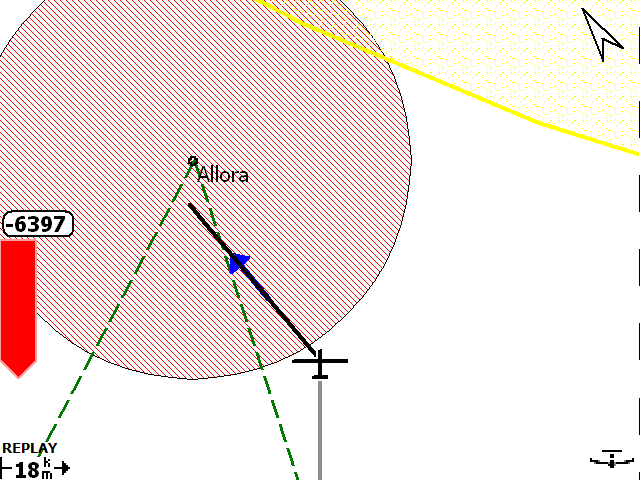
\includegraphics[angle=0,width=0.45\linewidth,keepaspectratio='true']{figures/faat01.png} & 
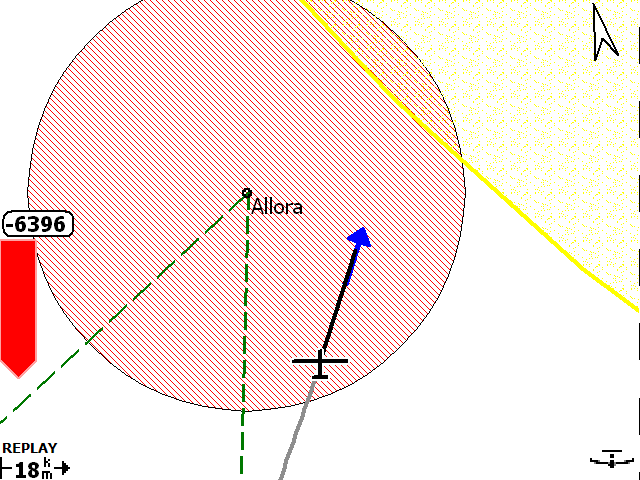
\includegraphics[angle=0,width=0.45\linewidth,keepaspectratio='true']{figures/faat02.png} \\
{\em Hors zone} & {\em Dans la zone} \\
Objectif (-20\%) sur la bissectrice & Objectif positionné sur la route \\

\midrule
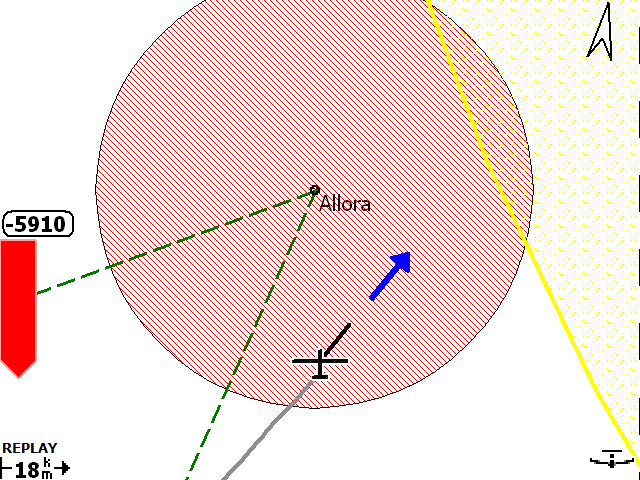
\includegraphics[angle=0,width=0.45\linewidth,keepaspectratio='true']{figures/faat03.png} & 
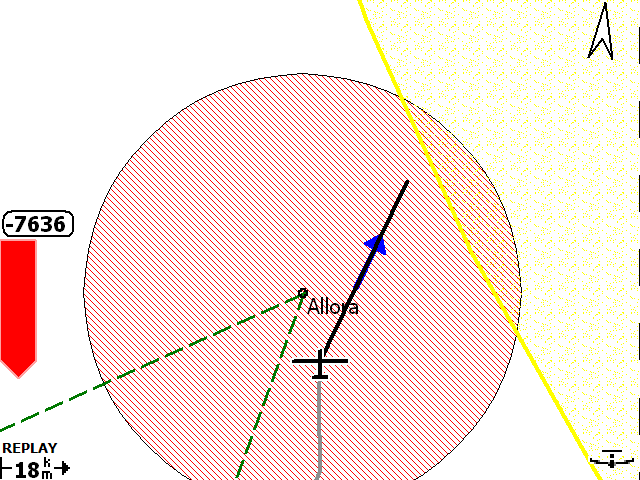
\includegraphics[angle=0,width=0.45\linewidth,keepaspectratio='true']{figures/faat04.png} \\
{\em Distance AAT diminuée par le pilote} & {\em Distance AAT augmentée par le pilote} \\
Objectif (-80\%) projeté sur la route & Objectif (80\%) projeté sur la route \\

\midrule
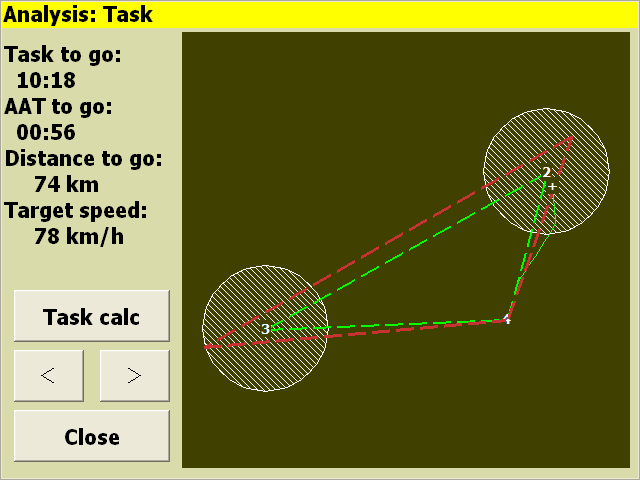
\includegraphics[angle=0,width=0.45\linewidth,keepaspectratio='true']{figures/faat05.png} & 
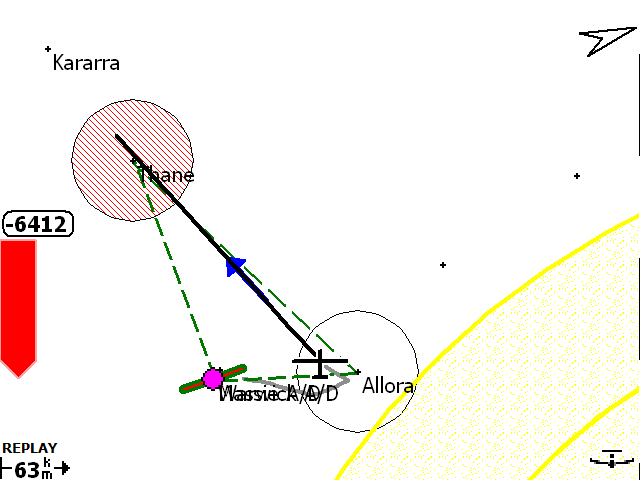
\includegraphics[angle=0,width=0.45\linewidth,keepaspectratio='true']{figures/faat06.png} \\
{\em Analyses (page circuit)} & {\em Prochain waypoint} \\
Chemin encadrant l'objectif  & "Préparer virage'' appuyé \\
\bottomrule
\end{longtable}
\end{center}
\end{maxipage}

\begin{maxipage}
\begin{center}
\begin{longtable}{|c|c|}
\toprule
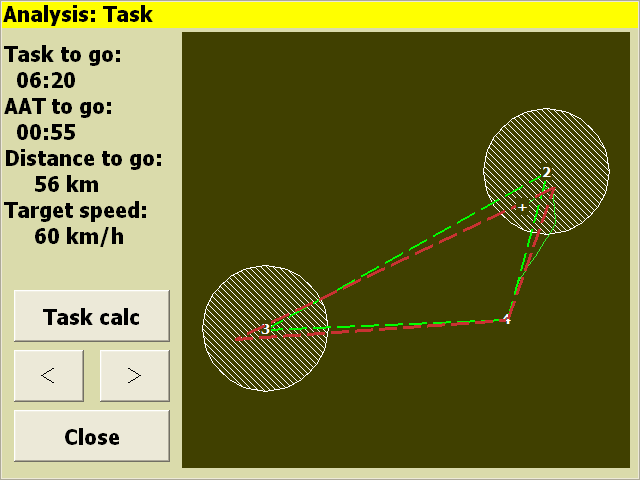
\includegraphics[angle=0,width=0.45\linewidth,keepaspectratio='true']{figures/faat07.png} & 
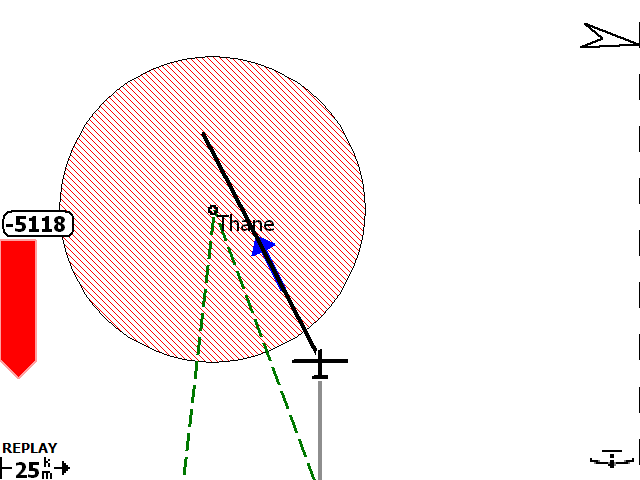
\includegraphics[angle=0,width=0.45\linewidth,keepaspectratio='true']{figures/faat08.png} \\
{\em Analyses (page circuit)} & {\em En approche de la prochaine zone} \\
Meilleur objectif calculé & Objectif (60\%) sur la bissectrice \\

\midrule
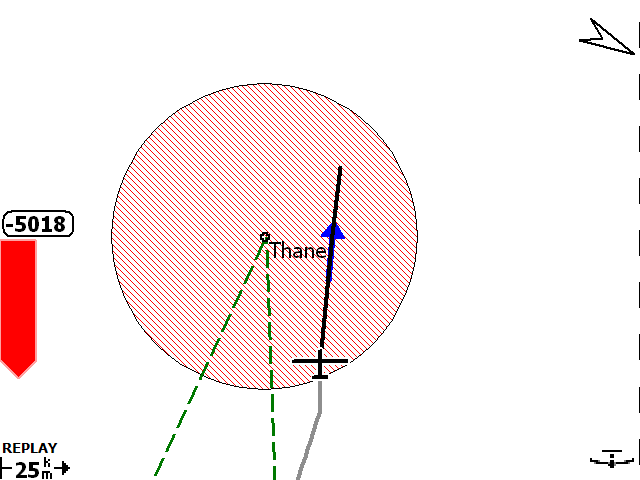
\includegraphics[angle=0,width=0.45\linewidth,keepaspectratio='true']{figures/faat09.png} & 
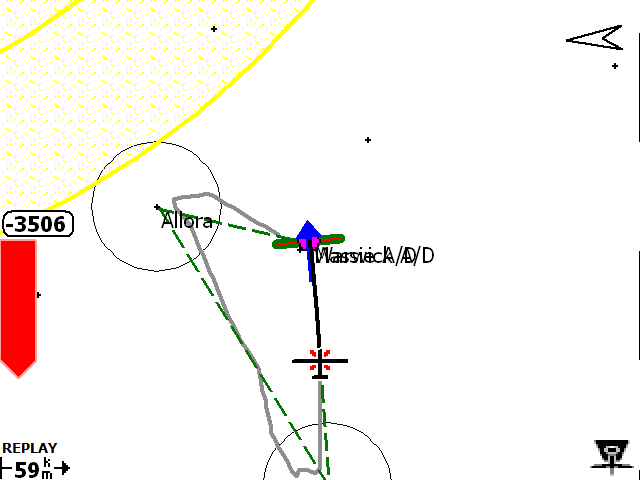
\includegraphics[angle=0,width=0.45\linewidth,keepaspectratio='true']{figures/faat11.png} \\
{\em Dans la zone} & {\em Prochain waypoint} \\
Objectif (60\%) projeté sur la route & "Préparer virage'' appuyé \\

\midrule
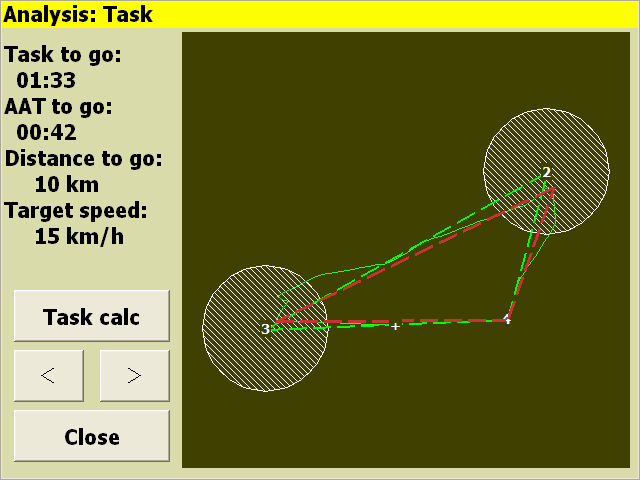
\includegraphics[angle=0,width=0.45\linewidth,keepaspectratio='true']{figures/faat12.png} &  \\
{\em Analyses (page circuit)} &  \\
Meilleurs objectifs calculés &  \\

\bottomrule
\end{longtable}
\end{center}
\end{maxipage}

\section{OnLine Contest}

Le menu Analyses contient la page "OLC Plus" pouvant être utilisée afin de voir le parcours optimal et le nombre de points estimés. Les paramètres de configuration \config{taskrules} (Valeurs par défaut du circuit) permettent de choisir l'ensemble de règles à appliquer pour l'optimisation OLC.

L'optimisation se fait en permanence et peut être consultée à volonté. Les pages Analyses affichent une vue du parcours optimisé, la distance et le score. Une infoBox donne aussi les valeurs instantanées OLC de distance et de score.

\begin{center}
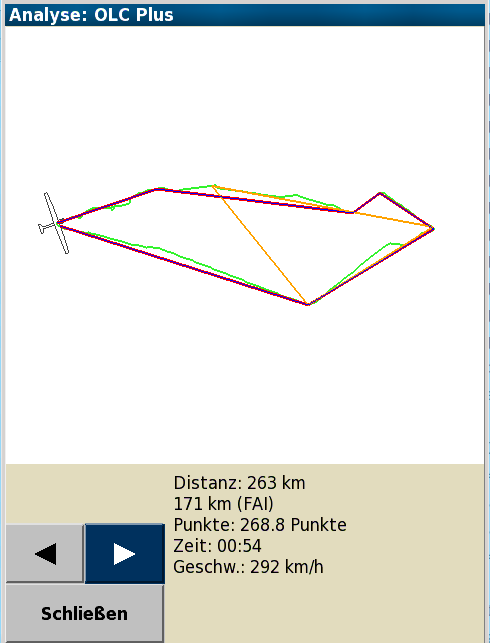
\includegraphics[angle=0,width=0.8\linewidth,keepaspectratio='true']{figures/shot-olc.png}
\end{center}

En vol OLC, les circuits AAT ou non AAT peuvent peuvent encore être utilisés pour la navigation. En vol, le calculateur optimise le vol en accord avec les règles OLC choisies.

Dans la page Analyses OLC la trace du planeur est représentée par une mince ligne verte tandis que le parcours optimal est représenté par une ligne rouge pointillée épaisse.

Si en finale le vol se poursuit, le score augmente et le résultat affiché est "en cours". Un ligne bleue montre le parcours projeté pour amélioré les résultats. Pour les type Sprint ou OLC classiques ce parcours est allongé dans la direction du waypoint courant. Pour les type OLC triangle, le parcours s'étend dans la direction permettant d'avoir le plus grand triangle possible.  \todonum{still true?}

Le résultat et la distance optimale sont approximatifs.

Une fois au sol les résultats ne sont plus mis à jour.


\section{Abandon/reprise et dégagements}

Si les conditions atmosphériques se dégradent, le pilote peut juger que l'épreuve ne peut être terminée. Dans cette situation il est possible d'abandonner l'épreuve et XCSoar aide le pilote à trouver un terrain posabe en sécurité.

\subsection*{Abandon du circuit}\label{sec:taskabort}
Le circuit est "abandonné" à la suite d'une de ces actions :
\begin{itemize}
\item Appui sur  \bmenug{Nav. 2}\blink\bmenug{Circuit Abandon}
\item Choix d'un terrain de dégagement dans la liste  \gesture{Bas - Gauche}
 \bmenug{Nav. 1}\blink\bmenug{Dégagmts}
\item Ou en sélectionnant une cible sur la carte et en démarrant un circuit "Aller à".
\end{itemize}

Une fois abandonné, tout type de circuit en cours est ignoré. La liste des points posables est ordonnée par ordre de proximité.

Le paramètre des options systèmes, "Polaire pour zone d'atteinte", permet de définir si le calcul des hauteurs d'arrivée en mode abandon utilise le calage MC juste avant l'abandon du circuit ou le calage MC de sécurité. \config{reachpolar} Par défaut le calage MC de sécurité est utilisé. Lors du passage en mode abandon, le calage MC utilisé est celui qui est le plus faible entre MC de sécurité et MC courant.

Les 10 points de virages les plus proches sont toujours affichés, même si aucun n'est posable.

Le point de virage actif, et en fait la liste des points posables les plus proches, est dynamique en mode abandon afin de présenter à tout moment plusieurs options d'atterrissage et que chaque option soit sélectionnable pour devenir un point de virage actif.\sketch{figures/abort-low.png}

Si les conditions météo s'améliorent le circuit peut être "repris" (\bmenug{Nav. 2}\blink\bmenug{Circuit Reprendre}). Le point de virage actif, avant l'abandon, est restauré ainsi que tous les détails du circuit qui était en cours. 

\subsection*{Dégagements} \label{sec:alternates}
Les terrains de dégagement sont mis à jour tout au long du vol. A la différence du mode "abandon", le mode "dégagements" permet d'avoir en permanence un œil sur les terrains posables les plus proches. Une liste de 6 terrains posables est actualisée. Ils sont triés à l'aide du paramètre 'Ordre des dégagements' (Simple, Circuit et Base). \config{alternatesmode} L'un de ces paramètres doit être en accord avec vos préférences.

La liste inclue le distance au point de dégagement, l'altitude pour l'atteindre et sa fréquence radio. Il y a aussi 2 infoBoxes dédiées aux 2 premiers éléments de la liste, de bons candidats à mettre dans une page d'infoBoxes supplémentaire.\sketch{figures/alternates_list.png}

Bien que les éléments de la liste des dégagements suivent des règles de fonctionnement différentes, ils ont le même comportement vis à vis du circuit en cours. Le choix d'un terrain de dégagement arrête le circuit en cours. Si les conditions s'améliorent le circuit peut être repris en utilisant le même bouton.

\section{Enregistrement}\label{sec:logger}

Un enregistreur de vol (logger) conforme aux règles IGC permet d'enregistrer les vols.

Avec XCSoar on peut accéder à plusieurs loggers :
\begin{itemize}
\item Un logger basé sur un logiciel. Toutes les versions de XCSoar proposent cette fonction. L'enregistreur est conforme aux standards IGC mais il n'est pas certifié.
\item Par exemple la version PRO d'Altair comporte un logger certifié IGC. XCSoar communique avec le logger comme avec tout autre appareil externe.
\item XCSoar peut aussi envoyer des déclarations de circuit vers des loggers externes. Pour que se soit possible il faut que l'appareil fasse partie de ceux de la liste des périphériques supportés (Configuration + Périph.). \config{comdevices}
\item  Pour certains parmi les nombreux loggers externes, XCSoar peut télécharger des fichiers IGC. Ceci est particulièrement pratique pour les loggers qui ne sont pas facilement démontables du planeur ou pour envoyer son fichier de vol si XCSoar est utilisé sur un smartphone.
\end{itemize}

\subsection*{Configuration}
Pour une matrice complète des fonctionnalités des loggers supportés, voir ~\ref{sec:supported-varios}.
La configuration est décrite en détails dans ~\ref{conf:logger}. Les détails du fichier de log se trouvent dans ~\ref{sec:logfiles}.

\subsection*{Activation de l'enregistreur}
La mise en route et l'arrêt de l'enregistreur peuvent être manuels ou automatiques. Pour les para-pentes XCSoar fourni seulement le démarrage automatique. Ainsi, une vitesse sol faible ou une hauteur faible au-dessus du relief ne stopperont pas l'enregistrement du vol. Si vous choisissez l'enregistrement automatique 'départ seulement' il faudra arrêter manuellement. Pour démarrer / arrêter manuellement, utiliser le menu :
\sketch{figures/logger-startdeclare.png}
\begin{quote}
\bmenug{Config. 2}\blink\bmenug{Enregistr. Démarrer}
\bmenug{Config. 2}\blink\bmenug{Enregistr. Arrêter}
\end{quote}

Quand le logger interne de XCSoar est en fonctionnement, un petit bouton rond vert, en bas et à droite, s'allume et s'éteint une fois par seconde.

Par défaut XCSoar est configuré en mode de démarrage et arrêt automatiques, l'enregistrement débute quand XCSoar détecte le début du vol et il s'arrête à l'atterrissage. La confirmation de démarrage d'enregistrement avec déclaration n'a lieu qu'en mode manuel : si le démarrage est automatique, la déclaration du circuit est aussi automatique. En mode simulation le logger ne peut être démarré automatiquement.

Si un circuit a été déclaré, alors toute tentative de modification du circuit fait apparaitre un message de confirmation qui invaliderai la déclaration du circuit. Ceci dans le but de rendre plus difficile de modifier involontairement le circuit, ce qui conduirai à un circuit déclaré invalide.

Le logger de XCSoar, quand il démarre, vérifie si il y a au moins 500kB d'espace libre pour stocker le circuit. Si il y a moins de 500kB de libre XCSoar élimine les plus anciens fichiers IGC. Il n'y a pas de message de confirmation. \warning

Le logger interne de XCSoar enregistre en permanence les 60 secondes passées. Ce qui fait qu'au décollage (automatique ou manuel) 60 secondes sont enregistrées avant le démarrage du logger. Le logger enregistre ainsi correctement la totalité du décollage.

\subsection*{Rejouer un enregistrement}\label{sec:logger-replay}
Les vols enregistrés au format IGC par XCSoar ou d'autres loggers peuvent être rejoués. On y accède par :
\begin{quote}
\bmenug{Config. 2}\blink\bmenug{Rejouer}
\end{quote}
\sketch{figures/loggerreplay.png}

Le mot "REPLAY" apparait en bas à gauche de l'écran et le programme se comporte comme si le GPS  recevait des informations de mises à jour.
Pour commencer à rejouer un vol, il faut choisir le fichier IGC à charger et ensuite appuyer sur \button{Démarrer} puis \button{Fermer}. La vitesse de défilement du vol peut être modifiée en modifiant le champ "Taux". Pour mettre en pause, mettre la valeur de "Taux" à zéro. Des valeurs de Taux élevées peuvent conduire à des valeurs dégradées de l'estimation du vent et autres fonctions de statistiques/analyses.

Pour arrêter de rejouer le vol, appuyer sur \button{Arrêter}.
Lorsqu'un vol est rejoué, le fait d'appuyer sur \button{Démarrer} redémarre le vol à son début.

\tip Il est recommandé de redémarrer l'appareil avant de voler, quand un fichier IGC a été rejoué, afin de resetter les paramètres de statistiques internes de XCSoar.

Quand on utilise XCSoar en mode FLY il n'est pas possible de rejouer un vol IGC si le GPS détecte que l'appareil est en mouvement.

Les fichiers IGC doivent avoir des intervalles de mesures assez réduits : 6 secondes ou moins sont des valeurs correctes pour rejouer les vols.


\subsection*{logger d'erreur}\label{sec:raw-logger}
Pour la faciliter la recherche de solution à des bugs du logiciel XCSoar il y a un enregistreur "brut". Si vous pouvez reproduire un comportement anormal du logiciel, il faut utiliser cet enregistreur. Démarrer l'enregistreur brut puis reproduisez le "bug" et arrêter l'enregistreur brut. Pour générer le fichier à envoyer aux développeurs de XCSoar :
\begin{quote}
\bmenug{Config. 3}\blink\bmenug{Logger brut}
\end{quote}
Pour corriger un bug, les développeurs ont besoin d'une description détaillée du problème et d'un fichier de traces comme celui généré par ce logger brut. Celui-ci permet d'accélérer énormément l'analyse de la cause du problème et donc de trouver sa solution et livrer rapidement une nouvelle version corrigée.

\section{Analyses du vol} \label{sec:analysis-climb}

Les pages Analyses sont très utiles pour planifier et gérer les vols sur la campagne. On y accède par le menu : 
 \gesture{Haut - Droite - Bas}
\begin{quote}
\bmenug{Info.}\blink\bmenug{Analyses}
\end{quote}

Plusieurs pages sont particulièrement intéressante :
\begin{description}
\item[Barographe]  Présente un graphique de l'altitude au cours du vol. Les statistiques sont exploitées pour évaluer la bande de travail (moyenne de la base et du sommet des ascendances) et pour donner une valeur estimée de la variation de plafond à court terme. La base et le plafond moyens des ascendances sont représentés par des lignes sur le graphe. 

Le bouton 'Paramètres' ouvre directement la page de configuration des paramètres du vol. Les valeurs des ballast, des moucherons, du QNH et de la température maximum peuvent être modifiées.

\begin{center}
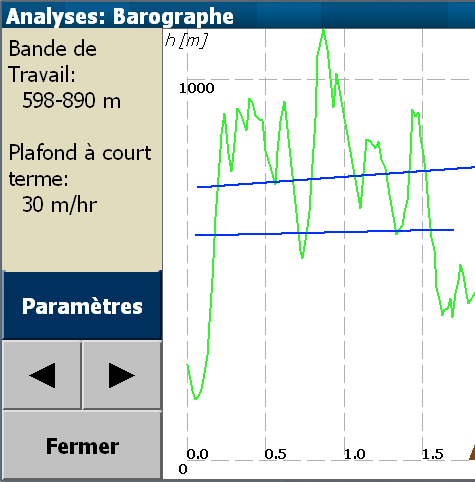
\includegraphics[angle=0,width=0.8\linewidth,keepaspectratio='true']{figures/analysis-barograph.png}
\end{center}

\item[Historique vario]
montre sous forme de graphique à barres la moyenne de chaque ascendance. Les statistiques sont utilisées pour calculer la moyenne générale et sa variation au cours du vol. La valeur du calage MC courant est affichée par une ligne rouge épaisse, la variation de la moyenne des ascendances par une ligne bleue.
Le bouton "Calc. circuit" permet d'ouvrir directement la page principale du gestionnaire de circuit et permet de faire varier le calage MC.

\begin{center}
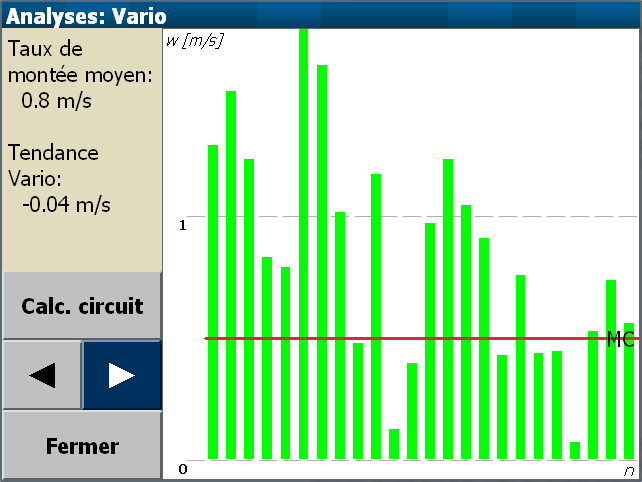
\includegraphics[angle=0,width=0.8\linewidth,keepaspectratio='true']{figures/analysis-climb.png}
\end{center}

\item[Circuit]
Cette page montre le parcours intégral du vol. Le circuit est représenté par une ligne verte épaisse en pointillé. Les zones AAT sont ombrées. Pour les circuits AAT le chemin restant depuis le planeur jusqu'au points de virages restants, est en pointillé rouge. Le parcours réalisé est représenté par une fine ligne continue verte.
  Le bouton 'Calc. circuit' ouvre directement le gestionnaire de circuit et permet de modifier le calage MC ou la longueur du circuit.

\begin{center}
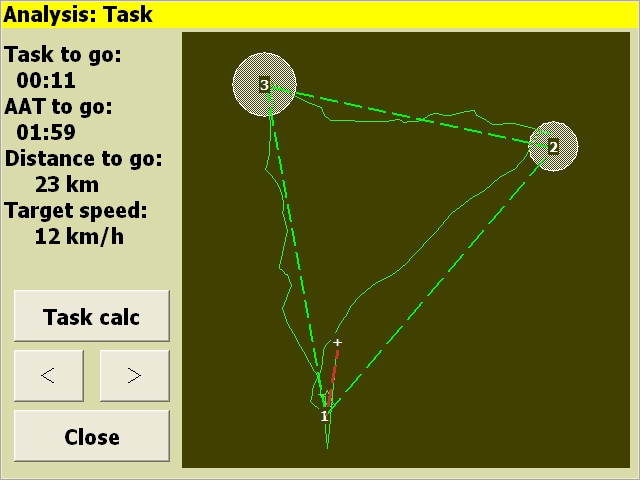
\includegraphics[angle=0,width=0.8\linewidth,keepaspectratio='true']{figures/analysis-task.png}
\end{center}

\end{description}

\section{Le coucher de soleil}

L'heure du coucher du soleil est consultable dans le panel "Times"  sous \bmenug{Info. 2}\blink\bmenug{Etats}. Notez que les conditions atmosphériques locales et l'environnement propre au terrain peuvent conduire à une visibilité très médiocre avant l'heure calculée du coucher de soleil.
Pour les PDA, l'heure d'été est paramétrée par le système d'exploitation du PDA. Pour Altair, le décalage de l'heure UTC, doit être réglé manuellement dans le panneau de configuration

 \bmenug{Config. 2}\blink\bmenug{Système}\blink\bmenug{Configuration}\blink\bmenug{Heure}.

Si l'heure d'arrivée prévue du circuit est après le coucher du soleil calculé, un message d'avertissement est affiché. 

